\task{Разрезания}
\begin{itemize}
\itA Поделим каждую из сторон квадрата на семь равных отрезков и рассмотрим 28 треугольников, получающихся, если соединить центр квадрата с краями каждого из этих отрезков. Все эти треугольники имеют одинаковую площадь (так как у них одинаковы основание и высота) и равные длины сторон, лежащие на сторонах квадрата (по построению).

Чтобы получить 7 многоугольников, требуемых в условии, объединим по четыре соседних треугольника.

\itB Смотреть рисунок:

\begin{center}
	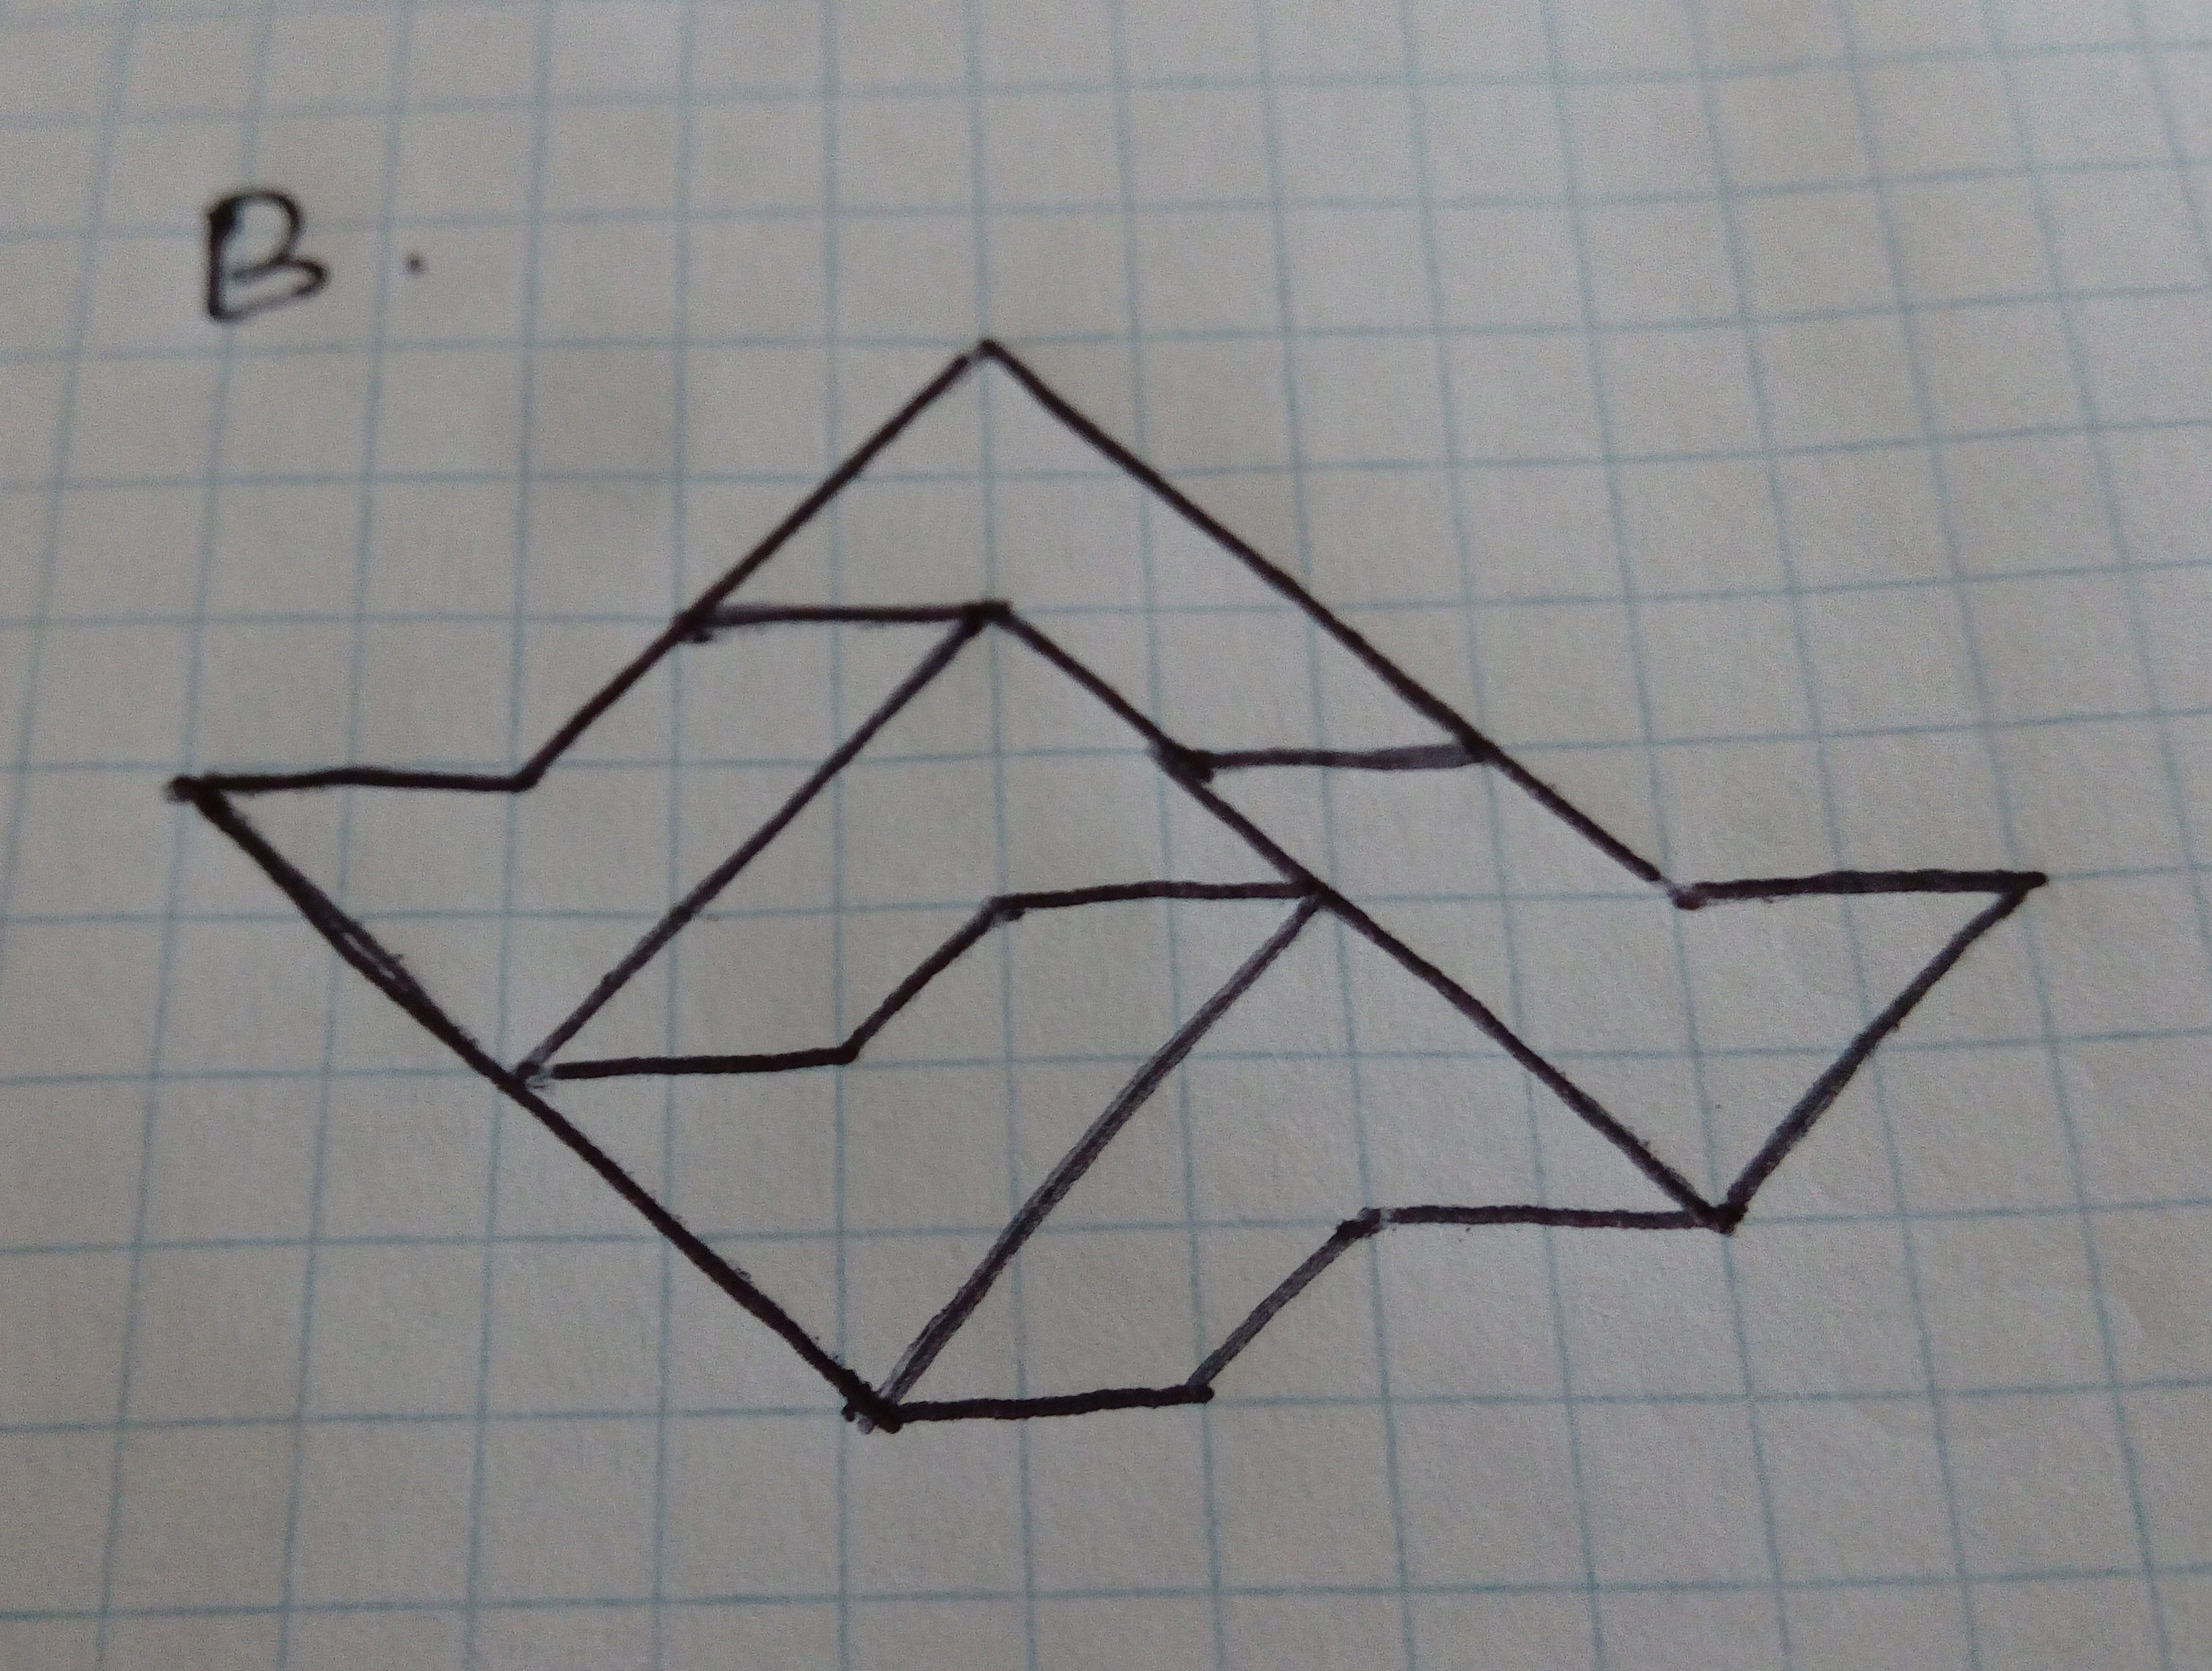
\includegraphics[natwidth=3081,natheight=2328,width=6cm]{figures/2018-figure-cuts}
\end{center}

\itC Аналогично тому, что было проделано в первом пункте данной задачи, мы умеем резать квадрат на три многоугольника равной площади с равной длиной сторон, лежащих на сторонах квадрата.

Разрежем каждый квадратный «слой» пирамиды на три таких многоугольника одинаковым образом (с точностью до подобия). Тогда в объединении всех слоёв получатся три многогранника одинакового объёма, несущие на себе одинаковое количество краски («выходящие» на стороны пирамиды одинаковой площадью своей границы).
\end{itemize}